\section{Geolocalización} % (fold)
\label{sec:geolocalizacion}
  La Geolocalización o Georreferenciación es un término bastante nuevo, de hecho no aparece en el diccionario de la Real Academia Española, no obstante se lo puede definir como:
% \footnote{http://dle.rae.es/}

  \begin{quote}
    El posicionamiento en el que se define la localización de un objeto espacial (representado mediante un punto, vector, área, volumen) en un sistema de coordenadas y datum determinado. Este proceso es utilizado frecuentemente en los Sistemas de Información Geográfica.\cite{Georreferenciacion}
  \end{quote}

  % Para entender esta definición se necesita explicar algunos términos

  La Georreferenciación antiguamente era bastantemente usada en el ámbito científico, y se necesitaba de instrumental y personal cualificado para su manejo, pero en la actualidad la cantidad de dispositivos con capacidad para geolocalizar un objeto sobre la tierra es bastante común, de hecho todos los smartphones actuales (en general los que se consideran gama media o alta) traen integrados receptores GPS (Global Position System), y sumados a la explosión de aplicaciones  que integran mapas con localización, ya que se puede tener una base de datos con coordenadas, descripciones, etc., que individualmente no aporta mucho valor pero al obtener datos de una gran cantidad de usuarios puede llegar a ser informacion valiosa ya que sirve para tomar decisiones a nivel de negocio, pero interpretar estos datos sería muy difícil sin la ayuda de los \emph{Sistemas de Información Geográfica}.\\

  Un \emph{SIG} es una herramienta que permite integrar, analizar, mostrar, interpretar y  entender las relaciones, patrones y tendencias de la información geográficamente referenciada \cite{what_is_gis}.
  % \footnote{http://www.esri.com/what-is-gis}
  Por estas razones es que actualmente existe una explosión de estas aplicaciones, donde empresas, particulares y hasta organismos gubernamentales están haciendo uso de estas tecnologías.
  Y las posibilidades son diversas, por ejemplo, si se quisiera planificar la construcción de un colegio se podría integrar los datos del censo con un mapa, identificando los sectores con mayor porcentaje de niños y localizando los sectores más propicios para realizar la construcción del inmueble. En el caso de una catástrofe natural, el tener las rutas de evacuación geolocalizadas y disponibles en un mapa de manera eficiente,  ayudaría en la evacuación de las personas del lugar.\\


  \subsection{Definiciones} % (fold)
  \label{sub:definiciones}

    En la aplicación desarrollada se requerirá trabajar con datos espaciales, y para ello es necesario entender algunos conceptos envueltos en el manejo de la información geográfica.

    \begin{description}
      \item[Coordenada:] Es una secuencia de n-números que designa la posición de un punto en un espacio n-dimensional. \\
      \item[Sistema de coordenadas:] Un sistema de coordenadas es  un conjunto de reglas matemáticas que especifican cómo las coordenadas son asignadas  a cada  punto.
      \item[Punto:] Es  la representación de una posición, topológicamente 0-dimensional (no tiene volumen, área, longitud o cualquier otra unidad multi-\\dimensional).
    \end{description}

    % \subsection{Coordenada} % (fold)
    % \label{sub:coordenada}
    %   Es una secuencia de n-números que designa la posición de un punto en un espacio n-dimensional. \\
    %   % one of a sequence of n-numbers designating the position of a point (4.17) in n-dimensional space
    %   % NOTA: En un
    %   % NOTE In a coordinate reference system, the numbers shall be qualified by units.

    % % subsection coordenada (end)

    % \subsection{Sistema de coordenadas} % (fold)
    % \label{sub:sistema_de_coordenadas}
    %   Un sistema de coordenadas es  un conjunto de reglas matemáticas que especifican cómo las coordenadas son asignadas  a cada  punto.
    %   % set of mathematical rules for specifying how coordinates (4.3) are to be assigned to each point (4.17)

    % % subsubsection sistema_de_coordenadas (end)
    % \subsection{Punto} % (fold)
    % \label{sub:punto}
    %   Es  la representación de una posición, topológicamente 0-dimensional (no tiene volumen, área, longitud o cualquier otra unidad multi-dimensional).
    %   % topological 0-dimensional geometric primitive (4.15), representing a position
    % % subsection punto (end)

    Estas definiciones están desarrolladas en la especificación \textbf{Simple Feature Access}, la cual es mantenida por la OGC (Open Geospatial Consortium). Esta especificación define el conjunto de tipos de datos (puntos, línea, polígono, etc) y las operaciones o métodos necesarios para manejar estos datos.

    % \footnote{\url{http://www.opengeospatial.org/standards/sfa}}

  % section definiciones (end)
  \subsection{Sistema de Coordenadas para datos Geográficos} % (fold)
  \label{sub:sistema_de_coordenadas_para_datos_geograficos}
    Se podría pensar en un sistema de coordenadas como la forma de dar sentido a un \emph{par de coordenadas}, por ejemplo cuando se ve una locación ``\verb|POINT(-66.1457475 -17.3937285)|'', cómo se interpretan estos números?.
    Podría ser la latitud y longitud del campus de la UMSS, o podría ser un sistema de anos luz desde alguna estrella en el Universo.
    El sistema de coordenadas es lo que diferencia estos casos.\\


    Una aplicación que maneja datos geográficos, generalmente trabaja con sistemas de coordenadas relacionadas con la superficie terrestre, conocidas como coordenadas espaciales (coordenadas globales), que permiten representar la tierra en \emph{3-Dimensiones} (3D), ya que esta es una Esfera (elipsoide oblato), o en una representación de la superficie terrestre en \emph{2-Dimensiones} (2D), se pueden nombrar los siguientes:

    \subsubsection{Coordenadas geocéntricas (X,Y,Z)} % (fold)
      \label{subs:coordenadas_geocentricas}
        También conocido como \emph{Coordenadas Cartesianas 3D}, Este sistema tiene como origen el centro de la Tierra, con el \emph{eje X} y el \emph{eje Y} en el plano del ecuador. El \emph{eje X} pasa a través del meridiano de Greenwich, y el \emph{eje Z}  coincide con el eje de rotación de la Tierra.

        \begin{figure}[H]
          \begin{center}
            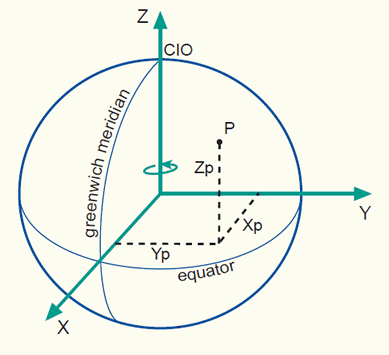
\includegraphics[width=0.7\textwidth]{coord_geocentric}
            \caption{Sistema de coordenadas Geocéntricas}
            \label{fig:coord_geocentric}
            \caption*{Fuente: \cite{coords2009} }
          \end{center}
        \end{figure}

        Este Sistema de coordenadas no es muy usado en la representación de datos, pero a veces se lo requiere para análisis de algoritmos y geometría computacional.
      % subsection coordenadas_geocentricas (end)

      \subsubsection{Coordenadas Geográficas} % (fold)
      \label{subs:coordenadas_geograficas}
        Sistema de coordenadas Geográfico, utiliza las coordenadas angulares latitud  (\emph{phi} o ${\phi}$) y longitud (\emph{lambda} o ${\lambda}$). Este sistema de coordenadas se expresa en grados, se lo puede representar con la forma \emph{grados:minutos:segundos }\verb|(17° 23' 37.4226" S, 66° 8' 44.691" W)|, o de la forma más común \emph{grados decimales} \verb|(-66.1457475 S, -17.3937285 W)|.\\

        El sistema de coordenadas  más ampliamente usado, el que usan por defecto los sistemas \emph{GPS}, es conocido como ``WGS 84'', y la mayoría de las aplicaciones que manejan mapas usan este sistema de coordenadas. Es el sistema que maneja los más ampliamente conocidos ``latitud y longitud''.\\

        \begin{figure}[H]
          \begin{center}
            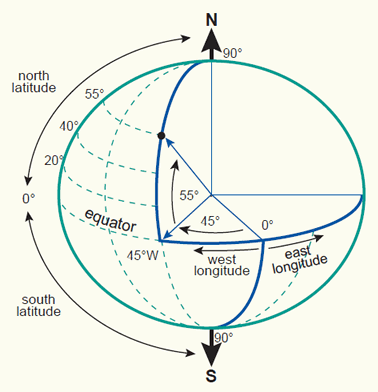
\includegraphics[width=0.7\textwidth]{coord_geographic}
            \caption{Sistema de coordenadas Geográficos}
            \label{fig:coord geographic}
            \caption*{Fuente: \cite{coords2009} }
          \end{center}

        \end{figure}

      % subsection coordenadas_geograficas (end)

      \subsubsection{Coordenadas Proyectadas} % (fold)
      \label{subs:coordenadas_proyectadas}
        Un sistema de coordenadas proyectadas es una representación plana y bidimensional de la  tierra. Se basa en un sistema de coordenadas \emph{geográficas esféricas}, pero utiliza unidades de \emph{medida lineales} para las coordenadas, de forma que los cálculos de distancia y área se pueden realizar en términos de esas mismas unidades.\cite{projected} \\

        Un sistema de coordenadas proyectadas requiere tomar la superficie esférica de la tierra y ``aplanarla'', este procedimiento se lo realiza con la finalidad de tener un mapa representable en una hoja de papel así como en la pantalla de la computadora. Sin embargo este procedimiento introduce diversos tipos de distorsión por lo que existen diferentes clases de proyecciones que varían según la región que se quiere representar de la Tierra.\\

        La proyección que usan \emph{Google Maps} y \emph{Open Street Maps} es la \textbf{Mercator Projection}\cite{gmaps_osm}, esta proyección está diseñada para preservar los ángulos y las formas de las líneas en forma recta, pero distorsiona los tamaños y las distancias mientras más lejos se encuentran de la línea del Ecuador. Esta proyección se puede apreciar en la figura \ref{fig:mercator_proyection}

% Google Maps usa la Proyección de Mercator para mostrar su mapa

        \begin{figure}[H]
          \begin{center}
            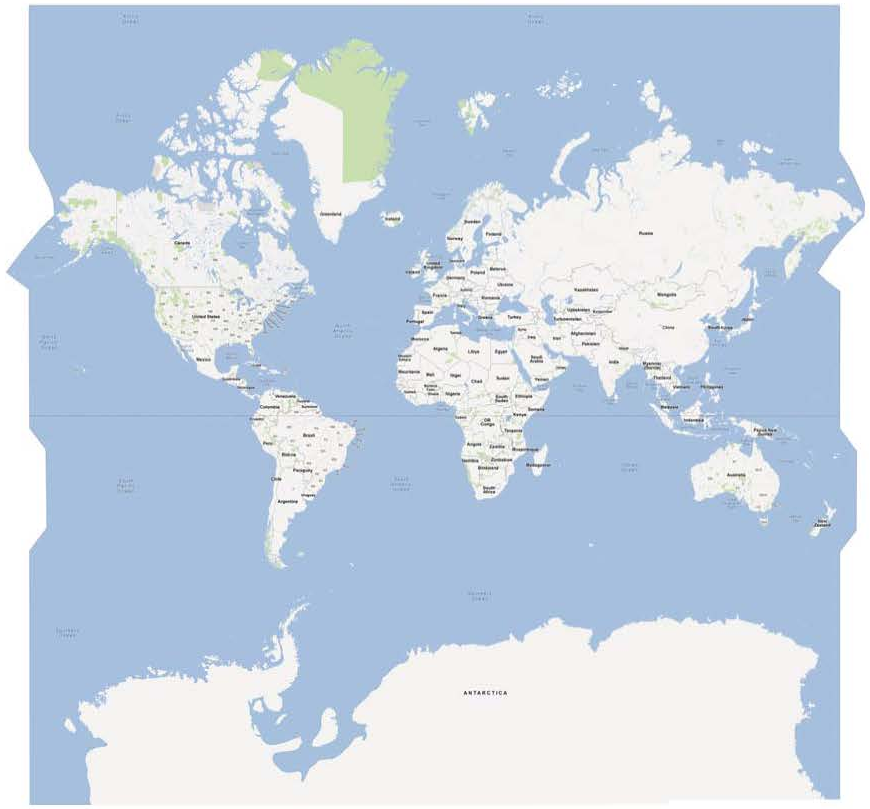
\includegraphics[width=0.6\textwidth]{mercator_proyection}
          \end{center}
          \caption{Sistema de coordenadas Proyectadas}
          \label{fig:mercator_proyection}
          \caption*{Fuente: \cite{coords2009} }
        \end{figure}

        Tal como se puede apreciar en la figura \ref{fig:mercator_proyection}, la distorsión de esta proyección se hace evidente si se observa la zona de Groenlandia ya que parecería tan grande como África o América del Sur, cosa que no es cierta, ya que Groenlandia es casi 14 veces más pequeño que África. A pesar de esta distorsión tan marcada, la \textbf{Proyección de Mercator} es una de las más usadas.
         % de hecho Google Maps usa esta proyección.
      % subsection coordenadas_proyectadas (end)

  %
  %     \subsection{Que se usó en la Aplicación} % (fold)
  %     \label{sub:que_se_uso_en_la_aplicacion}
  %       Es importante entender las diferencias entre los distintos tipos de sistemas de coordenadas porque computacionalmente realizar operaciones sobre los sistemas de coordenadas tiene un costo.
  %       Si se usara el sistema de coordenadas geográfico (WSG84) este es el más apropiado si se necesitaría usar grandes extensiones de la superficie terrestre, que al ser una estructura elipsoidal el costo computacional para realizar las operaciones matemáticas de calcular distancias, intersecciones, etc. es más elevado. En cambio el uso de un sistema de coordenadas proyectado (Mercator Projection) tiene un costo computacional más bajo, ya que se estaría trabajando con un sistema geométrico.\\
  %
  %       % Por otro lado,
  %       También hay tomar en cuenta la base de datos, ya que será esta la que se encargará de manejar los datos espaciales. Al estar usando PostGIS, se puede ver que en su documentacion\footnote{ http://postgis.org/documentation/manual-1.5/ch04.html} que claramente exorta el uso de un sistema geometrico sobre el uso de un sistema geografico si  se va trabajar con datos que cubran una pequena area geografica. Tomando en cuenta esta recomendación y el tamaño del área de estudio (el campus de la UMSS), se procedió a implementar en la base de datos el uso de la proyección Mercator. Se va usar Mercator sobre las otras proyecciones porque aparte de las ventajas que se mencionaron con anterioridad, Google Maps usa esta proyección y ya que se usará este mapa lo más correcto es trabajar con la misma proyección.
  %
  %
  %       % Comoprojected
  %       % PostGIS maneja dos tipos de datos, geográficos y geométricos
  %
  %     % section que_se_uso_en_la_aplicacion (end)
  % % section sistema_de_coordenadas_para_datos_geograficos (end)
  % % \section{Tipo de archivos} % (fold)
  % % \label{sec:tipo_de_archivos}
  % %
  % % section tipo_de_archivos (end)
  %
  % \subsection{Implementación} % (fold)
  % \label{sub:Implementacion}
  %   Para manejar datos georreferenciados con tecnología JavaScript, ya que se implementó el Backend con NodeJS, se hizo uso de la librería \textbf{KnexJS} para manejar la conexión a la base de datos PostgreSQL, y BookshelfJS para las consultas SQL pero para las consultas con datos geospaciales se realizó a través de esta herramienta pero usando la forma \emph{Raw SQL}\footnote{Raw SQL se refiere a consultas en ``SQL puro'' ya que el fuerte de BookshelfJS es el manejo de las consultas en forma de objetos (ORM), lamentablemente actualmente no existe mucho soporte para manejar datos geoespaciales}.
  %
  %   \begin{center}
  %     \begin{verbatim}
  %       var raw = "SELECT " +
  %                   " ST_AsGeoJSON(geom)::json As geometry," +
  %                   " name," +
  %                   " description," +
  %                   " phone," +
  %                   " level," +
  %                   " gid As id " +
  %                 " FROM place WHERE LOWER(name)
  %                        like LOWER('%" + name + "%')";
  %     \end{verbatim}
  %   \end{center}
  %
  %   De esta forma es que se recupera de la base de datos un lugar georreferenciado, donde este tiene un nombre, una descripción, un teléfono, el nivel o piso donde se encuentra pero lo importante de esta consulta es la obtención del ``punto'' geoespacial del lugar.
  %
  %   \begin{center}
  %     \begin{verbatim}
  %       "POINT (-66.14857015827988 -17.394421906929086)"
  %     \end{verbatim}
  %   \end{center}
  %
  %   % var raw = "SELECT seq, id1 AS node, id2 AS edge, cost
  %   %            FROM pgr_dijkstra('SELECT gid AS id,
  %   %                                     source::integer,
  %   %                                     target::integer,
  %   %                                     st_length(geom) AS cost
  %   %                               FROM public.ways', targetId, sourceId, false, false);";
  %
  %
  %    Este atributo es de tipo \emph{punto} o \emph{point} el cual tiene un \emph{SRID}\footnote{ Spatial Reference System Identifier, El \emph{SRID} corresponde a un sistema de referencia espacial basado en el elipsoide concreto usado para la creación de mapas de tierra plana o de tierra redonda.\cite{msdn_srid} } \emph{3857}\footnote{La proyección Mercator usa el EPSG 3857}, el SRID  es la llave primaria de la tabla \emph{spatial\_ref\_sys} que se crea cuando se inicializa una base de datos que soporte informacion geoespacial (PostGis), esta tabla provee la información necesaria para interpretar y convertir correctamente todas las coordenadas existentes, el \emph{SRID 3857} está definida en la tabla \emph{spatial\_ref\_sys} como ``Popular Visualisation CRS / Mercator''.\\
  %
  %
  %   Obtener la coordenada es el primer paso, seguidamente se debe mostrarlo sobre un mapa, en este caso \emph{Open Street Maps}, como se puede apreciar en la figura \ref{fig:ember_leaflet}, esta interfaz está implementada usando \emph{ember-leaflet}, el cual está principalmente diseñada para ofrecer una mejor experiencia de usuario en celulares smartphones.\\
  %
  %   % \begin{center}
  %   %   \begin{verbatim}
  %   %     var maker = new google.maps.Marker({
  %   %       position: new google.maps.LatLng( lat, lng  )
  %   %       map: UMSS.map
  %   %     });
  %   %   \end{verbatim}
  %   % \end{center}
  %
  %   \begin{verbatim}
  %     {{#leaflet-map lat=lat lng=lng zoom=zoom}}
  %       {{tile-layer url="http://{s}.tile.openstreetmap.fr/hot/{z}/{x}/{y}.png" }}
  %         {{#marker-layer location=location}}
  %           <h3>{{model.name}}</h3>
  %           {{model.description}} <br>
  %           <strong>telf:</strong> {{model.phone}} <br>
  %           <strong>piso </strong>#{{model.level}}
  %       {{/marker-layer}}
  %     {{/leaflet-map}}
  %   \end{verbatim}
  %
  %   \begin{figure}[H]
  %         \begin{center}
  %           \caption{\emph{ember-leaflet} nos ayuda a desplegar un mapa y mostrar un \emph{punto} o \emph{lugar} con un \emph{marcador} y dibuja una línea de color rojo sobre el mapa.}
  %           \label{fig:ember_leaflet}
  %           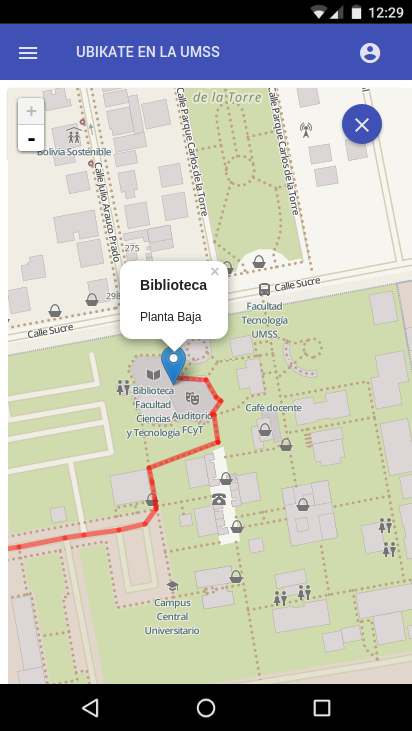
\includegraphics[width=0.5\textwidth]{ember_leaflet}
  %         \end{center}
  %         \caption*{Fuente: Elaboración propia.}
  %   \end{figure}
  %
  %

    % Pero esta coordenada  no sería  fácil de entender sin una adecuada representación sobre un mapa,


  % section Implementacion (end)
  % \section{Los datos} % (fold)
  % \label{sec:los_datos}


  %   Una vez implementada la Base de datos es necesario insertar ``los datos''
  % % section los_datos (end)


  % -------------------------------------------------------------------
  % -------------------------------------------------------------------
% -------------------------------------------------------------------

  % \section{Conclusión} % (fold)
  % \label{sec:geo_conclusion}
  %
    Los Mapas son herramientas muy útiles a la hora de desplegar información pero realizar el mapa, crear las fórmulas matemáticas con las cuales se trabajará, determinar cómo se usarán estas fórmulas para una representación adecuada de la superficie terrestre, es una tarea muy compleja. Como programador la tarea más complicada fue determinar el tipo de mapa y el sistema de coordenadas más adecuado para el tipo proyecto que se necesita desarrollar.\\

    Los términos de longitud y latitud son en un inicio, más fácilmente comprendidos que un sistema proyectado, pero no se puede tomar a la ligera una correcta comprensión del uso de los \emph{sistemas de coordenadas} en una base de datos espacial, un mal uso de estos conceptos puede generar errores a la hora de manejar datos  espaciales o en el resultado de las operaciones sobre estos  datos, llegando a resultados no deseados y que pueden costar más tiempo y dinero en una posterior corrección.\\

    La geolocalización es actualmente una tecnología y una herramienta usada en gran medida por una gran cantidad de aplicaciones web, añadiendo búsquedas y resultados personalizados a nivel país, ciudad, barrio y calle, resultando en una gran variedad de servicios y que actualmente es de gran ayuda en diferentes escenarios. La geolocalización nos ayuda a movernos por una ciudad, encontrar restaurantes, cines, transporte, etc. actualmente es una de las herramientas mas usadas y desarrolladas a nivel de industria, comercio, turismo, etc. y vale la pena estudiarla y entenderla.\\










% ************************************************************
    % Maps are deceivingly simple tools, and cartography a surprisingly complex discipline. While the most trouble many of us will have with a map is figuring out how to fold it, this simplicity belies great sophistication that has been developed over the years.
  % section geo_conclusion (end)


  % \begin{description}
  %   % \item[SIG] Un Sistema de Información Geográfica es una manera de visualizar como es y que está ocurriendo en algún lugar. La posibilidad de incorporar coordenadas con precisión.

  %   % A GIS is a collection of software, normally manipulated by its user through a single interface, and designed to perform a wide range of operations on geographic data.
  %   % Research  Methods in Geography
  %   % Basil Gomez and John Paul Jones III.
  %   % ISBN 978-1-4051-0710-5

  %   \item[Datum]
  %   \item[]
  %   \item[]
  % \end{description}

  % procesar
  % Se tien
  % , Sistema de Posicionamiento Global por sus siglas en espanol
% chapter geolocalizacion (end)
